\chapter{Project 1 Results --- Train a MiniGPT from Scratch}
\label{app:project1}

A 3.7M-parameter decoder-only Transformer was trained from scratch on 21.4\,MB of Project Gutenberg text (15 classic novels). Training used BPE ($V{=}2000$), context length 256, AdamW with warmup + cosine decay, and ran for 10K steps on an RTX 4090. Four ablation experiments isolate the impact of vocabulary size, architecture shape, context length, and learning rate.


\section{Baseline Training}

\begin{center}
\begin{tabular}{lr}
\toprule
Parameter & Value \\
\midrule
Layers / heads / d\_model & 4 / 4 / 256 \\
Parameters & 3,732,992 \\
Vocab size (BPE) & 2,000 \\
Context length & 256 \\
Peak LR & $3 \times 10^{-4}$ \\
Steps & 10,000 \\
Final val loss & 3.149 \\
Bits-per-byte & 1.509 \\
Wall time & $\sim$5 min \\
\bottomrule
\end{tabular}
\end{center}

\begin{figure}[ht]
\centering
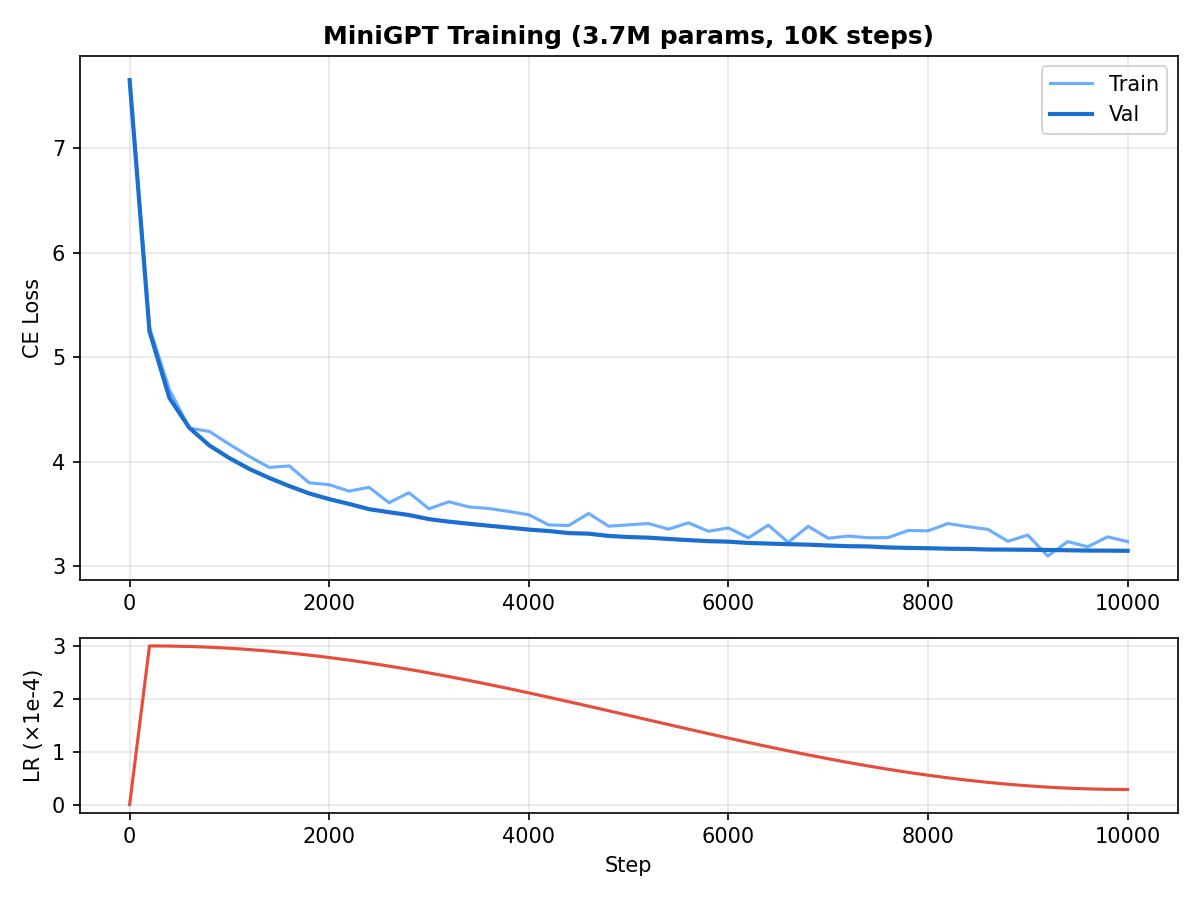
\includegraphics[width=0.85\textwidth]{projects/project1/figures/main_training.png}
\caption{Training and validation loss over 10K steps. Bottom panel shows the cosine learning-rate schedule with 200-step warmup.}
\label{fig:p1-training}
\end{figure}

The train--val gap is small (3.24 vs 3.15), indicating the model is still in the underfitting regime at this scale.


\section{Ablation 1: Vocabulary Size}

\textbf{Question:} Can we compare raw loss across tokenizers?

\begin{center}
\begin{tabular}{lrrrr}
\toprule
Config & Vocab & Bytes/Token & Raw Val Loss & Bits-per-Byte \\
\midrule
Char      &    65 & 1.03 & \textbf{1.18} & 1.653 \\
BPE-500   &   500 & 2.21 & 2.43 & 1.589 \\
BPE-2000  & 2{,}000 & 3.08 & 3.15 & 1.477 \\
BPE-8000  & 8{,}000 & 3.73 & 3.57 & \textbf{1.382} \\
\bottomrule
\end{tabular}
\end{center}

\begin{figure}[ht]
\centering
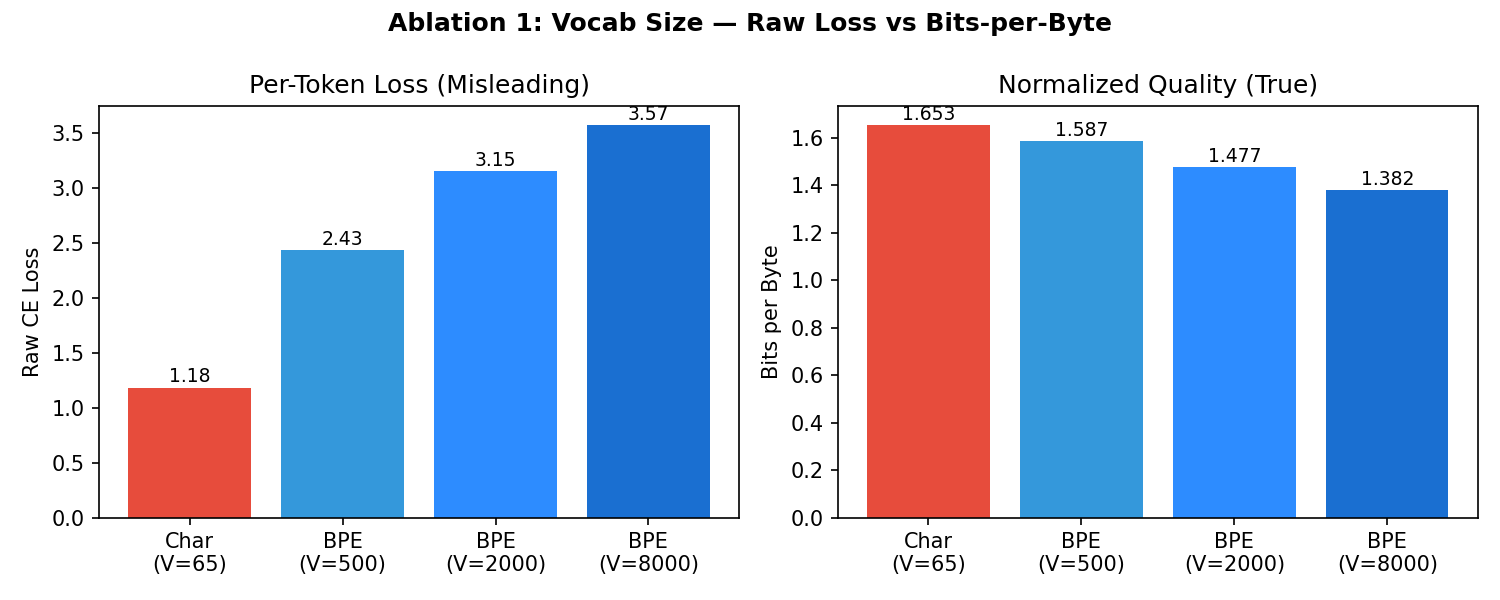
\includegraphics[width=0.9\textwidth]{projects/project1/figures/abl1_vocab.png}
\caption{Vocab size sweep: raw per-token loss (left) and bits-per-byte (right). Rankings are perfectly reversed---char-level appears best by raw loss but worst by the normalized metric.}
\label{fig:p1-vocab}
\end{figure}

\textbf{Finding:} Rankings are \emph{perfectly reversed}. Char-level shows the lowest raw loss (1.18) but the worst bits-per-byte (1.653). BPE-8000 has the highest raw loss (3.57) but the best normalized quality (1.382). Raw per-token loss is incomparable across tokenizers because the prediction task changes with vocabulary size.


\section{Ablation 2: Depth vs Width}

\textbf{Question:} At fixed $\sim$4M parameters, should we prefer deeper or wider models?

\begin{center}
\begin{tabular}{lrrrrr}
\toprule
Config & Layers & d\_model & Params & BPB & Wall Time \\
\midrule
Deep narrow   & 8 & 192 & 4.0M & 1.440 & 446\,s \\
Baseline      & 4 & 256 & 3.7M & 1.457 & 282\,s \\
Shallow wide  & 2 & 384 & 4.4M & \textbf{1.425} & \textbf{180\,s} \\
\bottomrule
\end{tabular}
\end{center}

\begin{figure}[ht]
\centering
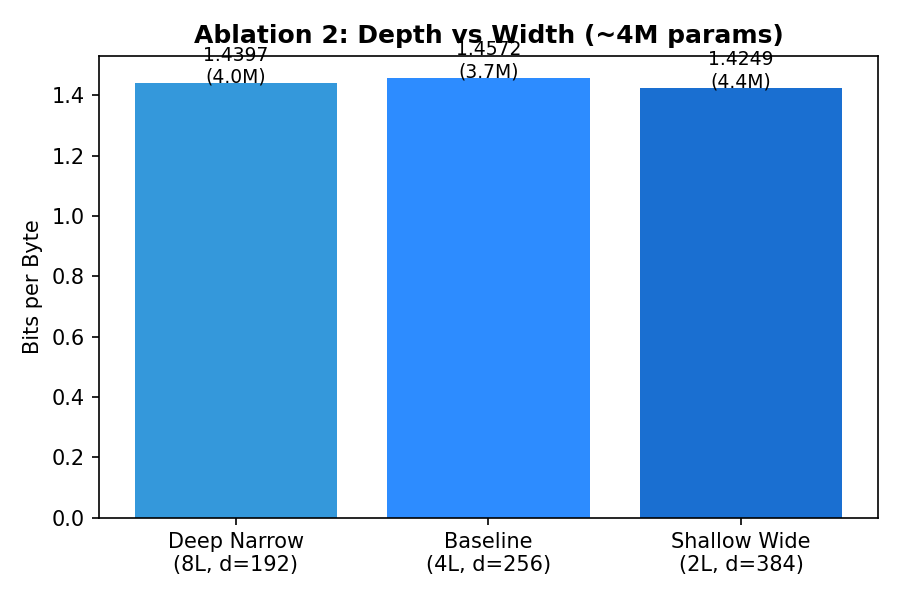
\includegraphics[width=0.6\textwidth]{projects/project1/figures/abl2_depth.png}
\caption{Depth vs width at $\sim$4M parameters. The 2-layer wide model wins on both quality and speed.}
\label{fig:p1-depth}
\end{figure}

\textbf{Finding:} At $\sim$4M scale, width wins. The 2-layer model (d=384) outperforms the 8-layer model (d=192) while training 2.5$\times$ faster. Each attention head in the wide model has d\_head=96 vs 48, giving it more per-head capacity. The compositional benefits of depth are not fully realized at this scale.


\section{Ablation 3: Context Length}

\textbf{Question:} How does context length affect quality and throughput?

\begin{center}
\begin{tabular}{rrrr}
\toprule
Context & BPB & Tokens/sec & Wall Time \\
\midrule
64  & 1.555 &  73K & 279\,s \\
128 & 1.506 & 139K & 295\,s \\
256 & 1.451 & 288K & 285\,s \\
512 & \textbf{1.411} & \textbf{438K} & 374\,s \\
\bottomrule
\end{tabular}
\end{center}

\begin{figure}[ht]
\centering
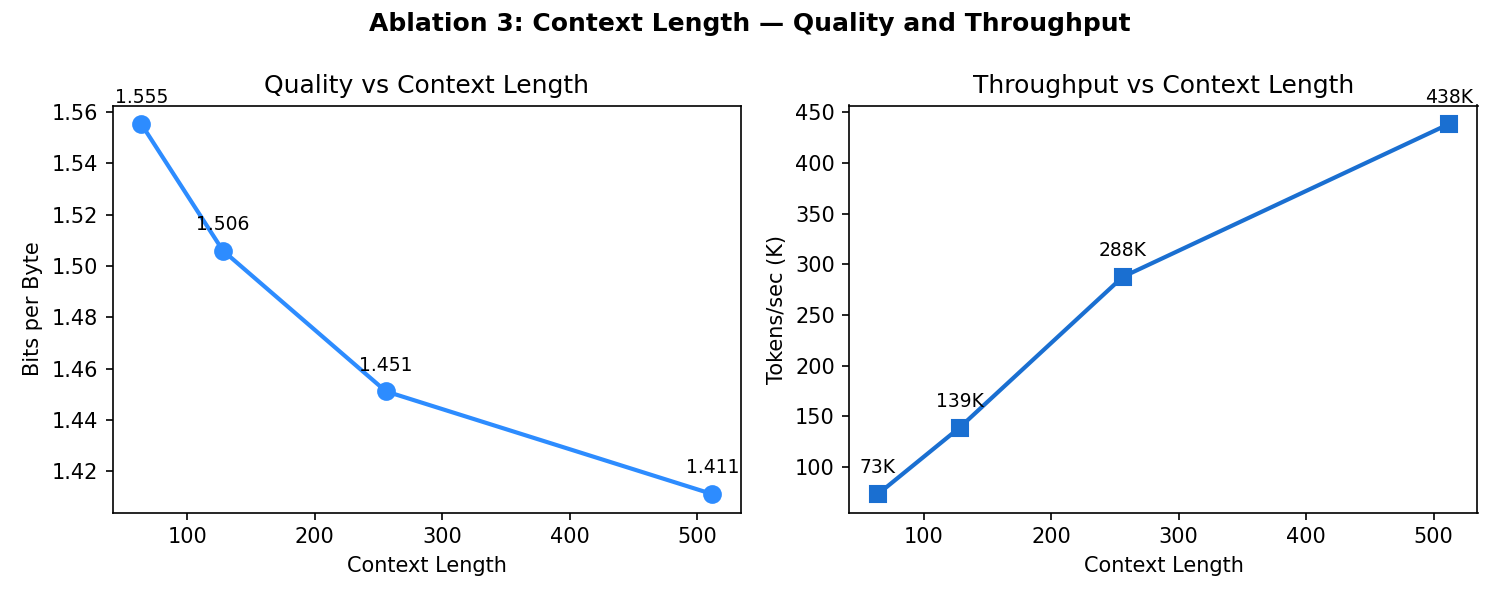
\includegraphics[width=0.9\textwidth]{projects/project1/figures/abl3_context.png}
\caption{Context length vs quality (left) and throughput (right). Both improve with longer context at this model scale.}
\label{fig:p1-context}
\end{figure}

\textbf{Finding:} Both quality and throughput improve with longer context. Throughput increasing with context length is counter-intuitive (attention is $O(T^2)$), but at 3.7M parameters the GPU is underutilized; longer sequences improve GPU saturation. This relationship reverses at larger model scales.


\section{Ablation 4: Learning Rate Sensitivity}

\textbf{Question:} How sensitive is training to the peak learning rate?

\begin{center}
\begin{tabular}{rrl}
\toprule
Peak LR & BPB & Note \\
\midrule
$10^{-5}$ & 2.238 & Severely undertrained \\
$10^{-4}$ & 1.598 & Underfitting \\
$3 \times 10^{-4}$ & 1.457 & Default \\
$10^{-3}$ & 1.404 & Better than default \\
$3 \times 10^{-3}$ & \textbf{1.401} & Best; no NaN \\
\bottomrule
\end{tabular}
\end{center}

\begin{figure}[ht]
\centering
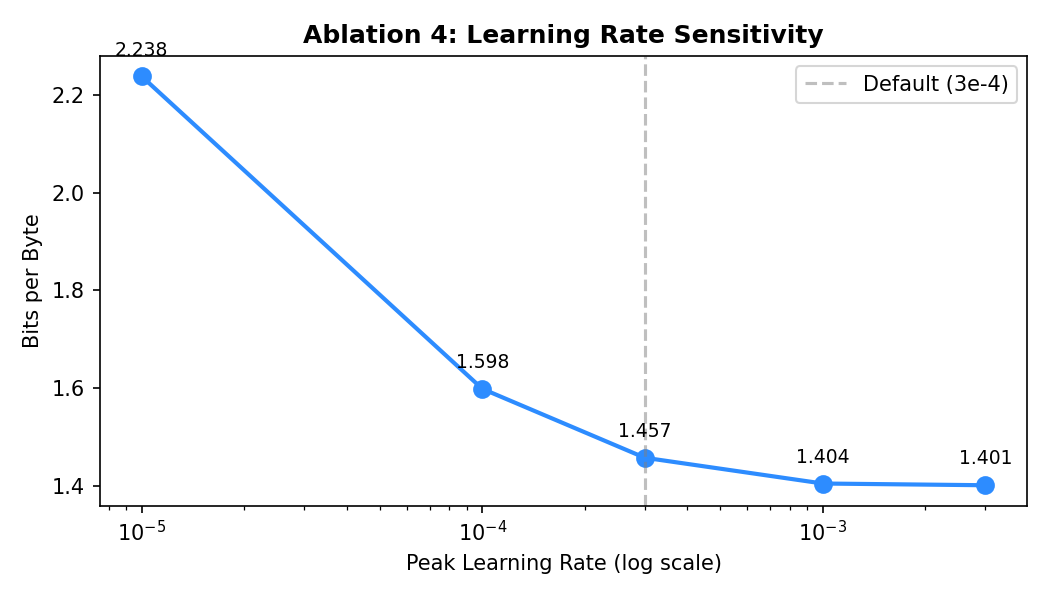
\includegraphics[width=0.65\textwidth]{projects/project1/figures/abl4_lr.png}
\caption{Learning rate sensitivity. The default 3e-4 (dashed line) is not optimal; 1e-3 and 3e-3 both produce better results without instability.}
\label{fig:p1-lr}
\end{figure}

\textbf{Finding:} The default LR ($3 \times 10^{-4}$) is not optimal. Higher LRs produce better results because this small model can tolerate aggressive updates, and gradient clipping prevents explosions. The gap between $10^{-5}$ and $10^{-4}$ (0.64 bpb) dwarfs the gap between $10^{-3}$ and $3 \times 10^{-3}$ (0.003 bpb): \textbf{undertrained is far worse than slightly aggressive.}


\section{Generation Samples}

Temperature controls the diversity--quality tradeoff. At $T{=}0.5$, output is grammatically correct but repetitive. At $T{=}0.8$, the model produces its best samples: coherent multi-sentence passages with character names and locations from the training corpus. At $T{=}1.2$, diversity increases but coherence degrades.

\begin{quote}
\small
\textbf{Prompt:} ``She looked at him and'' ($T{=}0.8$)

\textit{``She looked at him and Quincey suddenly, as though there were not the most cruel birds in life, and everything, would be done, in vain to be made tolerably go out of the desphysic. Vronsky knew how he wanted to speak to him\ldots''}
\end{quote}

The model has learned character names from the training corpus (Svidriga\"ilov, Vronsky, Zossimov from \emph{Crime and Punishment} and \emph{Anna Karenina}), French place names from \emph{Les Mis\'erables}, and dialogue formatting. It cannot maintain multi-sentence coherence---adjacent sentences are grammatically independent. This is expected for a 3.7M-parameter model.
